\documentclass[article,submit,pdftex,moreauthors]{Definitions/mdpi}
\usepackage{tikz}
\usepackage{pgf}
\usetikzlibrary{positioning, shapes, arrows.meta}

\firstpage{1} 
\makeatletter 
\setcounter{page}{\@firstpage} 
\makeatother
\pubvolume{1}
\issuenum{1}
\articlenumber{0}
\pubyear{2025}
\copyrightyear{2025}
\hreflink{https://doi.org/}

\Title{State of the Art: Summarization of RDF Graphs}
\TitleCitation{State of the Art: Summarization of RDF Graphs}

\Author{Raphael RAIMBAUD REMAZILLES $^{1}$, Diogo OLIVEIRA PEREIRA $^{2}$ and Oscar CORNEJO GUILLEN $^{3}$}
\AuthorNames{Raphael RAIMBAUD REMAZILLES, Diogo OLIVEIRA PEREIRA and Oscar CORNEJO GUILLEN}
\AuthorCitation{Raimbaud, R.; Oliveira, D.; Cornejo, O.}

\address{%
$^{1}$ \quad Affiliation 1; raphael.raimbaud-remazille@ens.uvsq.fr\\
$^{2}$ \quad Affiliation 2; diogo.oliveira-pereira@ens.uvsq.fr\\
$^{3}$ \quad Affiliation 3; oscar.cornejo-guillen@ens.uvsq.fr}

\corres{Correspondence: email@example.com; Tel.: +xx-xxxx-xxx-xxxx (F.L.)}

\abstract{This paper presents a state-of-the-art review of RDF graph summarization techniques, focusing on three recent research papers. The first section summarizes the key contributions of each study, while the second section provides a critical analysis of the strengths and weaknesses of the proposed approaches. Finally, potential research directions are discussed to address the limitations identified in existing methods.}

\keyword{Summarization; RDF Graphs; Centrality; Embeddings; SPARQL Queries}

\begin{document}

\section{Summary of the Papers}

The three papers reviewed introduce different approaches to RDF graph summarization. The first study focuses on selecting the most important nodes using centrality measures and a machine learning model. The goal is to generate a summarized version of the graph by selecting the \(k\) most frequently queried nodes. The challenge of linking selected nodes is addressed using approximation algorithms for the Steiner tree problem, minimizing the number of additional nodes required.

The second paper proposes an embedding-based approach (RDF2Vec) to identify key nodes and edges within an RDF graph. The authors use regression models to assign weights to nodes and edges and then apply approximation algorithms to interconnect the selected nodes. This method is evaluated on real-world datasets (DBpedia and Wikidata), demonstrating improvements in both efficiency and summarization quality compared to existing techniques.

The third study introduces a summarization method specifically designed to aid in SPARQL query formulation and optimization. It offers two types of summaries: a basic, quick summary and a refined, more complex but more precise summary. The authors define formal criteria to assess summary quality, such as representativeness and accuracy, and showcase their approach on real datasets.

The reviewed papers introduce three distinct approaches to RDF graph summarization. While each study adopts a different strategy, they all aim to generate concise yet informative representations of RDF graphs. The results indicate that embedding-based methods offer a scalable alternative to traditional centrality techniques, while query-oriented summarization provides a tailored view for specific query patterns.

\newpage
\subsection{Non-Quotient Structural Summarization using Embeddings}
In this summarization method, we integrate non-quotient structural methods with embedding-based node selection, thereby overcoming the scalability constraints of conventional centrality measures.

\paragraph{Step 1: RDF2Vec and Skip-Gram Embedding Generation}

RDF2Vec embeds the graph into sequences with four different walking strategies. The Random Walk strategy walks through neighboring nodes randomly, thereby keeping local connectivity intact. The Anonymous Walk removes node identities to highlight topological patterns. The HALK strategy adds a hierarchical dimension by including node attributes in the traversal process, while the N-Grams strategy identifies localized substructures by utilizing fixed-length node sequences.
Sequences are then processed by skip-gram, which learns embeddings by predicting context nodes in a sliding window. Properties (edges) are incorporated with entities in a unified 200-dimensional space and enable both semantic and structural comparison via \textbf{cosine similarity}.

\paragraph{Step 2: Assignment of Weights Using Regression Models}
Weight prediction is formulated as a regression task, based on the embeddings learned in the first phase. The machine learning methods are subsequently trained on weights which are derived from query logs later. Among models considered, Decision Trees (DT) achieve the best precision in predicting node weights. In contrast, Support Vector Regression (SVR) is good at predicting edges, with a significant outperformance over the SumMER method.

Other models, including Random Forests, AdaBoost, and Gradient Boosting, are tested, with differences in their performance depending on feature complexity and model architecture, such as tree depth and number of support vectors. By leveraging machine learning, this phase minimizes reliance on hand-crafted heuristics, allowing the model to learn implicit query patterns directly from usage data, rather than requiring pre-specified rules.

\paragraph{Step 3: Node Linking via Steiner Tree Approximations} In order to form solid connections among chosen nodes, the paper contrasts three approximations to the Steiner Tree problem. The first method, Minimum Spanning Tree (MST), builds a tree via either Kruskal's or Prim's algorithm, then prunes unnecessary leaves. The second method, SDIST, substitutes MST edges with shortest paths derived from Dijkstra's algorithm, prioritizing small edge weights to maximize relevance. Lastly, CHINS employs an incremental linking scheme, joining nodes by their closeness, starting from one seed node.

Of these techniques, SDIST with Kruskal's algorithm covers most. It effectively balances relevance of the path and computation. CHINS offers an intuitive linking procedure but has poor scaling, taking tens of thousands of seconds for big datasets like Wikidata, but SDIST takes less time. \\subsubsection*{Experimental Validation and Limitations} This systematic approach demonstrates that embedding-based summarization effectively balances semantic preservation and scalability. However, reducing log dependence and refining strategy selection to optimally fine-tune across diverse datasets remains an ongoing challenge.

\newpage

\subsection{Query-Oriented Summarization}

\subsubsection{\textbf{Baseline Summary}}

    \begin{figure}[H]
        \centering
        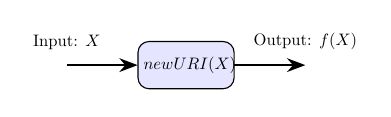
\begin{tikzpicture}[
            scale=0.6, % Reduce the overall scale of the TikZ diagram
            transform shape,
            block/.style={rectangle, draw, fill=blue!10, text width=1.8cm, text centered, rounded corners, minimum height=1cm},
            arrow/.style={thick, ->, >=Stealth}, % Arrows with arrowheads
            input/.style={coordinate},
            output/.style={coordinate}
        ]
        
        % Nodes
        \node[input] (inputX) {};
        \node[block, right=1.5cm of inputX] (PX) {$newURI(X)$};
        \node[output, right=1.5cm of PX] (output) {};
        
        % Labels
        \node[above=0.2cm of inputX] {Input: $X$};
        \node[above=0.2cm of output] {Output: $f(X)$};
        
        % Connections (Now with arrowheads)
        \draw[arrow] (inputX) -- (PX);
        \draw[arrow] (PX) -- (output);
        
        
        \end{tikzpicture}
        \caption{newURI() function block diagram}
        \label{fig:new_URI_function}
    \end{figure}

\vspace{0.5cm}

The Baseline Summary ($B_G$) provides a compact and simple representation of an RDF graph while maintaining representativeness and accuracy for query evaluation.

\subsubsection*{Steps:}

\begin{enumerate}
    \item \textbf{Input:} RDF Graph ($G$) containing schema and data properties.
    \item \textbf{Schema Preservation:} Retains the schema triples from $G$.
    \item \textbf{Creating Data Property Nodes:}
    \begin{itemize}
        \item For each data property $p$ in $G$:
        \begin{itemize}
            \item Assign a unique source node $S(p)$.
            \item Assign a unique target node $T(p)$.
            \item Add the triple $S(p) \ p \ T(p)$ to $B_G$.
        \end{itemize}
    \end{itemize}
    \item \textbf{Merging Sources and Targets:}
    \begin{itemize}
        \item If two properties share the same subject, they get the same source node.
        \item If two properties share the same object, they get the same target node.
        \item If an object of one property is the subject of another, they are merged.
    \end{itemize}
    \item \textbf{Class Assignments:}
    \begin{itemize}
        \item If a resource $s$ has a class $c$ in $G$, then $S(p)$ is assigned class $c$.
        \item If an object $o$ has a class $c$, then $T(p)$ is assigned class $c$.
    \end{itemize}
    \item \textbf{Handling Untyped Resources:}
    \begin{itemize}
        \item If a resource appears only in class assertions without properties, it gets a unique identifier.
    \end{itemize}
    \item \textbf{Output:} Baseline Summary Graph ($B_G$), a compact RDF summary maintaining schema, representativeness, and query accuracy.
\end{enumerate}

\subsubsection*{Complexity:}
The complexity of computing the Baseline Summary is $O(|G|^2)$.

\subsubsection*{More detailed rules}

\begin{figure}[H]
    \centering
    \includegraphics[width=0.7\linewidth]{images/This1.png}
    \caption{Baseline summary rules}
    \label{fig:summaryRules}
\end{figure}

\subsubsection{\textbf{Refined Summary}}

The Refined Summary ($R_G$) improves upon the Baseline Summary by reducing excessive merging of nodes, leading to better accuracy.

\subsubsection*{Steps:}

\begin{enumerate}
    \item \textbf{Input:} RDF Graph ($G$).
    \item \textbf{Schema Preservation:} Schema triples are copied from $G$.
    \item \textbf{Creating Data Property Nodes with Refinement:}
    \begin{itemize}
        \item For each data property $p$:
        \begin{itemize}
            \item Assign source and target nodes more selectively.
            \item Preserve distinct nodes unless necessary to merge them.
        \end{itemize}
    \end{itemize}
    \item \textbf{More Selective Merging:}
    \begin{itemize}
        \item Only merge property sources and targets when their resources \textbf{lack explicit types}.
        \item If resources have explicit types, separate nodes are created for each distinct type.
    \end{itemize}
    \item \textbf{Class Assignments with Better Differentiation:}
    \begin{itemize}
        \item Assigns types carefully to prevent unnecessary generalization.
        \item Improves query accuracy by maintaining distinctions between different resource types.
    \end{itemize}
    \item \textbf{Output:} Refined Summary Graph ($R_G$), a more accurate summary compared to $B_G$.
\end{enumerate}

\subsubsection*{Complexity:}
The complexity of computing the Refined Summary is $O(|G|^5)$.

\subsubsection{\textbf{Example}}

\begin{figure}[H]
    \centering
    \includegraphics[width=0.5\linewidth]{images/This2.png}
    \caption{RDF Graph Sample}
    \label{fig:summaryExamples1}
\end{figure}

\begin{figure}[H]
    \centering
    \includegraphics[width=0.8\linewidth]{images/This3.png}
    \caption{$B_G$}
    \label{fig:summaryExamples2}
\end{figure}

\begin{figure}[H]
    \centering
    \includegraphics[width=\linewidth]{images/This4.png}
    \caption{$R_G$}
    \label{fig:summaryExamples3}
\end{figure}

\section{Critical Analysis}

\begin{table}[H]
\raggedright
\caption{Strengths and Weaknesses of the Proposed Approaches}
\resizebox{0.9\textwidth}{!}{
\begin{tabular}{|p{4cm}|p{5cm}|p{5cm}|}
\toprule
\textbf{Approach} & \textbf{Strengths} & \textbf{Weaknesses} \\
\midrule
\textbf{Centrality and Machine Learning} & 
\begin{itemize}
    \item Uses a variety of centrality measures.
    \item Incorporates machine learning techniques.
\end{itemize} &
\begin{itemize}
    \item Relies on query logs to define ideal summaries.
    \item High complexity due to the Steiner tree problem.
\end{itemize} \\
\midrule
\textbf{Embedding-Based Summarization} & 
\begin{itemize}
    \item Captures graph semantics through embeddings.
    \item Reduces computational cost compared to centrality-based measures.
\end{itemize} &
\begin{itemize}
    \item Depends on query logs for training models.
    \item Limited to two knowledge bases (DBpedia and Wikidata).
\end{itemize} \\
\midrule
\textbf{Query-Oriented Summarization} & 
\begin{itemize}
    \item Optimized for SPARQL query performance.
    \item Flexible with two summarization types (basic and refined).
\end{itemize} &
\begin{itemize}
    \item High complexity of refined summary (\(O(|G|^5)\)).
    \item Dependent on the quality of the RDFS schema.
\end{itemize} \\
\bottomrule
\end{tabular}
}
\end{table}

\subsection{Potential Research Directions to Address Limitations}

\begin{itemize}
    \item \textbf{Hybrid Structural and Semantic Approach}
    
    \item \textbf{Multi-Level Summarization}
    
\end{itemize}

\paragraph{\textbf{Hybrid Structural and Semantic Approach}}

This next section presents our hybrid approach to RDF graph summarization, which integrates structural centrality measures with semantic embeddings to generate high-quality summaries of knowledge graphs. Our approach addresses the limitations of purely structural or purely semantic methods by combining their strengths.

\subsection{System Architecture}
Our system architecture consists of four main components: (1) Data Acquisition, (2) Structural Analysis, (3) Semantic Embedding, and (4) Summary Generation. Figure~\ref{fig:architecture} illustrates the overall architecture of our system.

\begin{figure}[H]
    \centering
    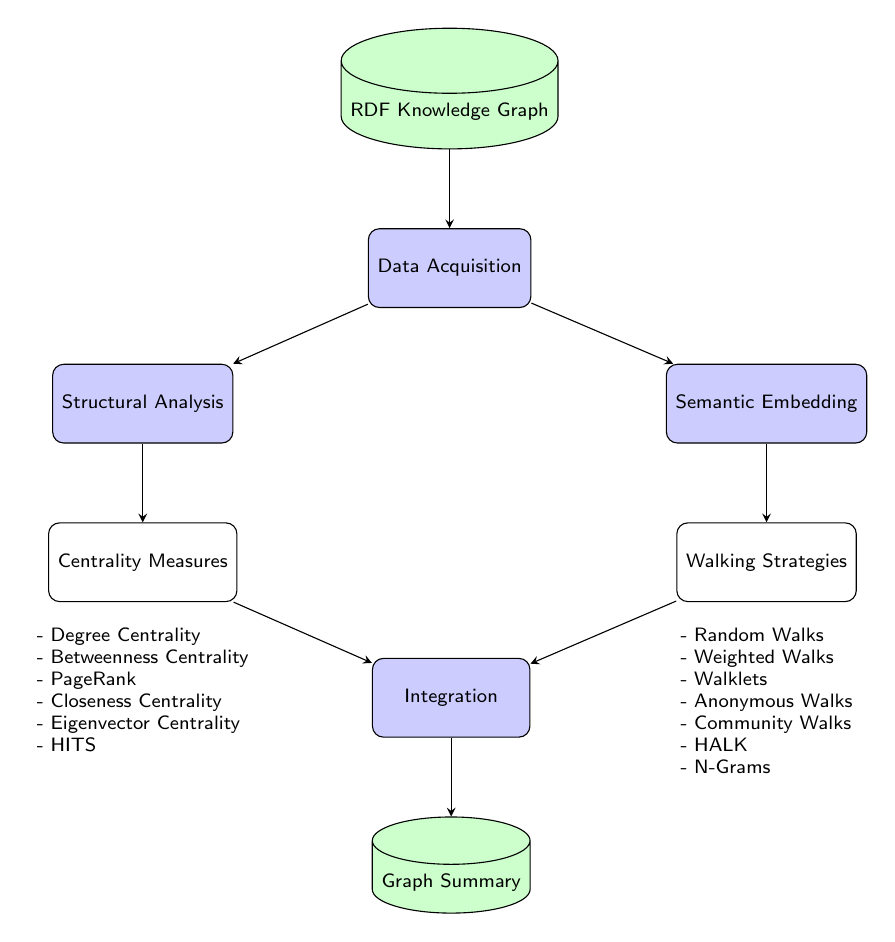
\begin{tikzpicture}[
        node distance=1cm,
        box/.style={rectangle, draw, rounded corners, minimum width=2cm, minimum height=1cm, text centered, font=\scriptsize\sffamily},
        arrow/.style={->, >=stealth, thin},
        process/.style={rectangle, draw, fill=blue!20, rounded corners, minimum width=2cm, minimum height=1cm, text centered, font=\scriptsize\sffamily},
        data/.style={cylinder, draw, shape border rotate=90, aspect=0.3, fill=green!20, minimum height=1cm, minimum width=2cm, text centered, font=\scriptsize\sffamily},
        decision/.style={diamond, draw, fill=orange!20, minimum width=2cm, minimum height=1cm, text centered, font=\scriptsize\sffamily}
    ]

    \node[data] (input) {RDF Knowledge Graph};
    
    \node[process, below=of input] (acquisition) {Data Acquisition};
    
    \node[process, below left=of acquisition, xshift=-1cm] (structural) {Structural Analysis};
    \node[process, below right=of acquisition, xshift=1cm] (semantic) {Semantic Embedding};
    
    \node[box, below=of structural] (centrality) {Centrality Measures};
    \node[box, below=of semantic] (walking) {Walking Strategies};
    
    \node[process, below right=of centrality, xshift=1cm] (integration) {Integration};
    
    \node[data, below=of integration] (summary) {Graph Summary};
    
    \draw[arrow] (input) -- (acquisition);
    \draw[arrow] (acquisition) -- (structural);
    \draw[arrow] (acquisition) -- (semantic);
    \draw[arrow] (structural) -- (centrality);
    \draw[arrow] (semantic) -- (walking);
    \draw[arrow] (centrality) -- (integration);
    \draw[arrow] (walking) -- (integration);
    \draw[arrow] (integration) -- (summary);
    
    \node[below=of centrality, yshift=0.8cm, align=left, font=\scriptsize\sffamily] {
        - Degree Centrality\\
        - Betweenness Centrality\\
        - PageRank\\
        - Closeness Centrality\\
        - Eigenvector Centrality\\
        - HITS
    };
    
    \node[below=of walking, yshift=0.8cm, align=left, font=\scriptsize\sffamily] {
        - Random Walks\\
        - Weighted Walks\\
        - Walklets\\
        - Anonymous Walks\\
        - Community Walks\\
        - HALK\\
        - N-Grams
    };
    
    \end{tikzpicture}
    \caption{System architecture of the hybrid structural and semantic approach to RDF graph summarization.}
    \label{fig:architecture}
\end{figure}

The Data Acquisition component retrieves RDF data from various sources, including Wikidata, and constructs a graph representation. The Structural Analysis component calculates multiple centrality measures to identify structurally important nodes. The Semantic Embedding component generates vector representations of nodes using RDF2Vec with different walking strategies. Finally, the Summary Generation component combines the structural and semantic information to produce a compact summary of the knowledge graph.

\subsection{Structural Centrality Measures}
We implement and evaluate eight different centrality measures to capture various aspects of node importance in the RDF graph:

\subsubsection{Degree Centrality}
Degree centrality measures the number of edges connected to a node. In directed graphs, we distinguish between in-degree (incoming edges) and out-degree (outgoing edges) centrality. For an undirected graph $G = (V, E)$, the degree centrality of a node $v \in V$ is defined as:

\begin{equation}
C_D(v) = \frac{deg(v)}{|V| - 1}
\end{equation}

where $deg(v)$ is the degree of node $v$ and $|V|$ is the number of nodes in the graph.

\subsubsection{Betweenness Centrality}
Betweenness centrality measures the extent to which a node lies on the shortest paths between other nodes. It is defined as:

\begin{equation}
C_B(v) = \sum_{s \neq v \neq t} \frac{\sigma_{st}(v)}{\sigma_{st}}
\end{equation}

where $\sigma_{st}$ is the number of shortest paths from node $s$ to node $t$, and $\sigma_{st}(v)$ is the number of those paths that pass through node $v$.

\subsubsection{PageRank}
PageRank measures the importance of a node based on the importance of its neighbors. It is defined recursively as:

\begin{equation}
PR(v) = \frac{1-d}{|V|} + d \sum_{u \in N_{in}(v)} \frac{PR(u)}{|N_{out}(u)|}
\end{equation}

where $d$ is a damping factor (typically 0.85), $N_{in}(v)$ is the set of nodes that link to $v$, and $N_{out}(u)$ is the set of nodes that $u$ links to.

\subsubsection{Closeness Centrality}
Closeness centrality measures how close a node is to all other nodes in the graph. It is defined as:

\begin{equation}
C_C(v) = \frac{|V| - 1}{\sum_{u \neq v} d(v, u)}
\end{equation}

where $d(v, u)$ is the shortest path distance between nodes $v$ and $u$.

\subsubsection{Eigenvector Centrality}
Eigenvector centrality assigns importance to nodes based on the importance of their neighbors. It is defined as the principal eigenvector of the adjacency matrix of the graph.

\subsubsection{HITS (Hub and Authority Scores)}
HITS assigns two scores to each node: a hub score and an authority score. Hub nodes point to many good authorities, while authority nodes are pointed to by many good hubs. The scores are calculated iteratively until convergence.


\subsection{Semantic Embedding Generation}
We use RDF2Vec to generate semantic embeddings for nodes in the RDF graph. RDF2Vec adapts the Word2Vec algorithm to RDF graphs by first generating random walks on the graph and then applying Word2Vec to learn vector representations of nodes.

\subsubsection{Walking Strategies}
We implement and evaluate seven different walking strategies to explore their impact on embedding quality:

\begin{enumerate}
    \item \textbf{Random Walks}: Standard random walks starting from each entity.
    \item \textbf{Weighted Walks}: Random walks where the probability of choosing an edge is proportional to its weight.
    \item \textbf{Walklets}: Multi-scale random walks that capture relationships at different scales.
    \item \textbf{Anonymous Walks}: Walks that preserve structural information while anonymizing node identities.
    \item \textbf{Community Walks}: Walks that are biased to stay within communities.
    \item \textbf{HALK (Hierarchical Alternative Walks)}: Walks that capture hierarchical relationships in the graph.
    \item \textbf{N-Grams}: Walks that capture sequential patterns in the graph.
\end{enumerate}

\subsubsection{Embedding Training}
After generating walks, we train a Skip-gram model to learn vector representations of nodes. The Skip-gram model predicts the context (surrounding nodes) given a target node. The objective function is:

\begin{equation}
\max_\theta \sum_{(w, c) \in D} \log P(c | w; \theta)
\end{equation}

where $D$ is the set of all word-context pairs in the walks, $w$ is the target word, $c$ is the context word, and $\theta$ are the model parameters.

\subsection{Integration of Structural and Semantic Information}
We propose a hybrid approach that effectively combines structural centrality measures with semantic embeddings to create comprehensive node importance scores. This integration enhances the quality of the resulting graph summaries by leveraging both the network topology and the semantic relationships between entities.

\subsubsection{Feature Fusion}
Our implementation fuses structural and semantic features through a machine learning model. This approach processes multiple centrality measures alongside embedding-based features:

\begin{equation}
    I(v) = ML(C_1(v), C_2(v), \ldots, C_n(v), E_1(v), E_2(v), \ldots, E_m(v))
\end{equation}

where $I(v)$ is the importance score of node $v$, $C_i(v)$ are centrality measures, $E_j(v)$ are embedding-derived features, and $ML$ is a machine learning model that predicts the overall importance.

\subsubsection{Weighted Importance Score}
In addition to machine learning fusion, we implement a weighted combination approach that allows explicit control over the relative importance of structural versus semantic components:

\begin{equation}
    I(v) = \alpha \cdot S(v) + (1-\alpha) \cdot M(v)
\end{equation}

where $S(v)$ is a normalized structural score derived from centrality measures, $M(v)$ is a semantic score derived from embeddings, and $\alpha \in [0,1]$ is a weighting parameter that controls the balance between structural and semantic information. By default, we set $\alpha = 0.7$, giving slightly more weight to structural features while still incorporating semantic information.

\subsubsection{Embedding-Enhanced Centrality Measures}
We extend traditional centrality measures by incorporating semantic information. For example, our implementation of Semantic PageRank computes edge weights based on cosine similarity between node embeddings:

\begin{equation}
    w(u, v) = \frac{\text{cos}(e_u, e_v) + 1}{2}
\end{equation}

where $w(u, v)$ is the weight of the edge from node $u$ to node $v$, and $e_u$ and $e_v$ are the embeddings of nodes $u$ and $v$, respectively. The transformation $\frac{x+1}{2}$ ensures that edge weights are positive, as required by the PageRank algorithm.

\subsubsection{Semantic Diversity Measure}
We introduce a novel semantic diversity measure that quantifies how unique a node is within the embedding space:

\begin{equation}
    D(v) = 1 - \frac{1}{|V|-1} \sum_{u \neq v} \text{cos}(e_v, e_u)
\end{equation}

This measure assigns higher scores to nodes that have embeddings dissimilar to other nodes, thereby identifying entities that represent unique concepts or fill specific semantic roles in the knowledge graph.

\subsection{Node Selection Algorithm}
To select the most important nodes for inclusion in the summary, we employ a machine learning approach that combines multiple regression models. The algorithm processes structural and semantic features to predict node importance and selects the top-$k$ nodes based on these predictions.

\subsubsection{Machine Learning Models}
We evaluate several regression models for predicting node importance:

\begin{itemize}
    \item \textbf{Gradient Boosting Trees}: Combines multiple decision trees to improve prediction accuracy.
    \item \textbf{Random Forests}: Ensemble learning method using multiple decision trees.
    \item \textbf{Linear Regression (OLS)}: Predicts importance as a linear combination of features.
    \item \textbf{Ridge Regression}: Linear regression with L2 regularization.
    \item \textbf{ElasticNet}: Linear regression with a combination of L1 and L2 regularization.
\end{itemize}

These models are evaluated using cross-validation, and the best-performing model is selected for the final node importance prediction.



\bibliographystyle{IEEEtran}
\bibliography{references}


\newpage

\authorcontributions{Conceptualization, X.X. and Y.Y.; methodology, X.X.; software, X.X.; validation, X.X., Y.Y., and Z.Z.; formal analysis, X.X.; investigation, X.X.; resources, X.X.; data curation, X.X.; writing—original draft preparation, X.X.; writing—review and editing, X.X.; visualization, X.X.; supervision, X.X.; project administration, X.X.; funding acquisition, Y.Y. All authors have read and agreed to the published version of the manuscript.}

\funding{This research received no external funding.}

\institutionalreview{Not applicable.}

\informedconsent{Not applicable.}

\dataavailability{No new data were created or analyzed in this study. Data sharing is not applicable to this article.}

\acknowledgments{The authors would like to thank the reviewers for their valuable feedback.}

\conflictsofinterest{The authors declare no conflicts of interest.}

\abbreviations{Abbreviations}{
The following abbreviations are used in this manuscript:\\
\noindent 
\begin{tabular}{@{}ll}
RDF & Resource Description Framework\\
SPARQL & SPARQL Protocol and RDF Query Language\\
KG & Knowledge Graph\\
\end{tabular}
}

\end{document}
